\documentclass[11pt]{report}
\usepackage[margin=0.5in]{geometry}
\usepackage{mathpazo}
\usepackage{amsmath}
\usepackage[colorlinks=true]{hyperref}
\usepackage{parskip}
\usepackage{tikz}

\title{ECE 457C Spring 2022 Course Review}
\author{Saif K.}

% Make lists condensed %
\usepackage{enumitem}
\setlist{nosep}

% images come from subfolder
\graphicspath{images/}

\begin{document}

\maketitle

\chapter{Reinforcement Learning}
This section aims to describe what reinforcement learning is and is not.

RL is simultaneously:
\begin{itemize}
	\item A class of problems
	\item A set of solution methods that work well on the problem
	\item The field that studies the above two things
\end{itemize}

RL involves an \textbf{agent} interacting with an \textbf{environment} over time to achieve some \textbf{goal}. It does so by balancing the \textbf{exploitation} of actions it knows to be good with the \textbf{exploration} of actions it has less information about, but which may be more fruitful in the long run.

RL is \textbf{not} supervised learning. The latter involves:
\begin{itemize}
	\item A training set of appropriate labels given data, generated by some expert
	\item An agent which \textbf{generalizes} from this to incorporate new data
\end{itemize}
In `uncharted territory,' the first point is impractical, and the second is unlikely to achieve the goal.

RL is \textbf{not} unsupervised learning. The latter involves inferring some structure in unlabeled data. This may be \textit{useful} in achieving the goal in some environment, but is not \textit{sufficient} to do so.



\chapter{Multi-Armed Bandits}
The k-armed bandit problem involves k slot machines each of which produces some reward according to a (hidden) probability distribution. The goal of the agent is to maximize its reward by selecting an arm to pull in each timestep.

Because the rewards for machine $j$ follow a probability distribution (which may or may not be \textbf{stationary}), we can define the `value' of selecting it as

\begin{equation}
	\label{eqn:k-bandit-value}
	q_\ast(a_j) = \mathbb{E}[R_t | A_t = a_j] \ \ \ \ \forall j \in \mathbb{Z}, 0 \leq j < k
\end{equation}

% todo: ensure optimal-q function is written
Note the analogy to the optimal value function \autoref{eqn:optimal-q}

\section{Action-Value Methods}\label{par:Action-Value Methods}

\begin{equation}
	\label{eqn:k-bandit-Q-est}
	Q_t(a) = \frac{\sum_{i=1}^{t-1} R_i \mathbb{1}_{A_i=a}}{\sum_{i=1}^{t-1}\mathbb{1}_{A_i=a}}
\end{equation}

One way to estimate $q_\ast$, shown in \autoref{eqn:k-bandit-Q-est}, is to replace the expectation in \autoref{eqn:k-bandit-value} with an average over the actions taken. Note that this is a simple example of a \textbf{Monte-Carlo} method described in \autoref{sec:Monte-Carlo Methods}. This estimate is not necessarily the best, but it is guaranteed to converge in the limit so long as all actions are selected infinitely often.

Given an estimate, how should we perform action selection?
\begin{itemize}
	\item Greedy: $A_t = \text{argmax}_{a}(Q_t(a)) = A_t^\ast$
	\item Epsilon-Greedy: choose $A_t^\ast$ with probability $1-\epsilon$, otherwise randomly select \textbf{any} action
\end{itemize}

\section{Incremental Implementation}\label{par:Incremental Implementation}
\begin{equation}
	\label{eqn:k-bandit-incremental-implementation}
	Q_{n+1} = Q_{n} + \frac{1}{n}\left(R_n - Q_n\right)
\end{equation}

Where $Q_{n}$ is the estimate $Q_t(a)$ for the action selected at time $t$, which gave reward $R_n$. This is simply a running average, but demonstrates the basic form that many tabular algorithms use to update the $Q$ estimate:

\begin{equation}
	\label{eqn:target-update-equation}
	\text{New Value} \xleftarrow{} \text{Old Value} + \text{StepSize}\cdot\left(\text{Target} - \text{Old Value}\right)
\end{equation}

\begin{itemize}
	\item The value in brackets (Target - Old) is called the \textbf{error} term
	\item StepSize may \textbf{not} be constant over time, for example in \autoref{eqn:k-bandit-incremental-implementation} it depends on the number of times the action has been taken by time $t$
\end{itemize}


\section{Nonstationary Problems}\label{par:Nonstationary}
\begin{equation}
	\label{eqn:k-bandit-nonstationary}
	Q_{n+1} = Q_{n} + \alpha\left(R_n - Q_n\right)
\end{equation}

A constant step-size parameter weights recent rewards more than old rewards and is thus a neat way of performing an update in a non-stationary environment. As an exercise, if you express \autoref{eqn:k-bandit-nonstationary} as a sum you will see that reward $R_i$ is weighted by $\alpha(1-\alpha)^{n-i}$.

\section{Optimistic Initial Values}
\begin{itemize}
	\item A trick to encourage exploration - set all the initial estimates high so that the agent will only switch off them if it continually gets `disappointed' by them
	\item Works well on stationary k-bandit, but is \textbf{not} a general way to encourage exploration
\end{itemize}

\section{Upper-Confidence Bound}\label{sec:UCB}
\begin{equation}
	\label{eqn:UCB}
	A_t = \text{argmax}_{a}\left[ Q_t(a) + c \sqrt{\frac{\ln{t}}{N_t(a)}}\right]
\end{equation}

The idea here is to improve on $\epsilon$-greediness by favouring actions that are more likely to be better in the $\epsilon$ case, which depends on two things:
\begin{itemize}
	\item The current estimate of the action
	\item The uncertainty in that estimate
\end{itemize}

Correspondingly, UCB selection has the following properties:

\begin{itemize}
	\item $N_t(a)$ indicates the number of times action $a$ has been selected by time $t$
	\begin{itemize}
		\item The higher this is, the \textit{less} uncertainty there is in the estimate $Q_t(a)$, hence it is in the denominator
		\item By convention, if $N_t(a)=0$, we consider it a maximizing action
	\end{itemize}
	\item $\ln{t}$ increases over time \textit{monotonically}, thus increasing the probability of selection for actions that are not selected over time. This ensures that all actions will eventually be selected regardless of the initial estimates
	\item $c$ is (confusingly) the confidence level - the higher it is the less confident we are in estimates, since we weight the variance term higher
	\item It is called Upper-Confidence bound since the $c\sqrt{\cdot}$ term is the upper bound on the estimate of $a$
\end{itemize}



\section{Gradient-Bandit Algorithms}
\begin{equation}
	\label{eqn:gradient-bandit}
	P[A_t = a] = \frac{e^{H_t(a)}}{\sum_{b=1}^k e^{H_t(b)}} \equiv \pi(a)
\end{equation}

In this approach, we simply represent the policy by recording a number $H \in \mathbb{R}$ known as the `preference' for each action, which has no interpretation in terms of the reward. The function in \autoref{eqn:gradient-bandit} simply turns these values into a valid probability distribution in a nice way - this is also known as the \textit{softmax} distribution. The question is how to learn these values, and the answer is given by the \textbf{stochastic gradient ascent} algorithm:

\begin{align}
	\label{eqn:bandit-stochastic-gradient}
	H(A_t) &\xleftarrow{} H(A_t) + \alpha(R_t - \bar{R}_t)(1-\pi_t(A_t))\\
	H(a) &\xleftarrow{} H(a) + \alpha(R_t - \bar{R}_t)\pi_t(a) \ \ \ \ \ \ \forall a \neq A_t
\end{align}

% todo: ensure the policy gradient refernce
Where $\bar{R}_t$ is the average of all the rewards up to but not including $t$. This is an instance of a stochastic gradient algorithm that uses a \textbf{baseline}, which comes up again in section \autoref{sec:policy-gradient}


\chapter{Finite MDPs}
Markov Decision Processes, or MDPs, are a formalism for describing the types of problems we would like to solve in RL. A finite MDP involves an \textbf{agent} interacting with an \textbf{environment}. There is a finite set $\mathcal{S}$ of states that the environment can be in (which includes the state of the agent). There is a finite set $\mathcal{A}$ (which may be dependent on the state) of actions the agent can take. There is a finite set $\mathcal{R} \subset \mathbb{R}$ of rewards the agent will receive for taking that action. Time evolves in discrete steps $t = 0, 1, 2...$, and at each point the agent takes some action. The \textbf{trajectory} of an agent is thus:

\begin{equation}
	\label{eqn:mdp-trajectory}
	S_0, A_0, R_1, S_1, A_1, R_2, ...
\end{equation}


The \textbf{Markov property} states that the distribution of $S_t$ and $R_t$ depend only on the previous state and action. That is, if an environment is \textbf{`markovian'}, we can write down a distribution known as the \textbf{dynamics} of the environment:

\begin{equation}
	\label{eqn:mdp-dynamics}
	p(s', r | s, a) \equiv Pr\{S_t = s', R_t = r | S_{t-1} =s, A_{t-1} = a\}
\end{equation}

It is a fundamental hypothesis of RL that everything we mean by `goal' and `purpose' can be thought of as the maximization of $\mathbb{E}[\sum_{t=0}{R_t}]$. There is considerable power in selecting exactly how to define a reward to achieve some goal. For example, when trying to win a game, we should give a reward for winning. When trying to minimize the steps taken to win the game, there should be a negative reward for each step it takes.

\section{Return}
Many tasks are \textbf{episodic} in that the task ends at $t=T$. In these cases, we define a \textbf{return}. In the episodic case this can simply be the sum of rewards until the episode end, however in the case of continuing tasks we need the sum to be finite and thus add a factor $0 \le \gamma \le 1$ known as the \textbf{discounting factor}:

\begin{equation}
	G_t = \sum_{k=0}^{\infty} \gamma^kR_{t+k+1} = R_{t+1} + \gamma G_{t+1}
\end{equation}

\section{Policies and Value Functions}
Almost all RL algorithms involve learning value functions which indicate \textit{how good} it is to be in a given state or perform an action in a given state. This is defined in terms of the expected return (or expected future discounted reward) that we would get in a given situation.

Since the expected return depends on how the agent will act in the future, reward is also computed with respect to a \textbf{policy}, which can be described as a function $\pi(a|s)$ that gives the probability of taking an action in a state. The policy an agent uses may change over time.

The state value is given by
\begin{equation}
	\label{eqn:state-value}
	v_\pi(s) \equiv \mathbb{E}_\pi[G_t | S_t = s] = \mathbb{E}_\pi\left[\sum_{k=0}^{\infty} \gamma^k R_{t+k+1} | S_t = s \right]
\end{equation}

The state-action (or just action) value is given by
\begin{equation}
	\label{eqn:state-action-value}
	q_\pi(s,a) \equiv \mathbb{E}_\pi[G_t | S_t = s, A_t = a] = \mathbb{E}_\pi\left[\sum_{k=0}^{\infty} \gamma^k R_{t+k+1} | S_t = s, A_t = a \right]
\end{equation}

Note that in the expectation, the sequence $R_t$ depends on $\pi_t$ (or just $\pi$ if the policy is constant) through the \textbf{dynamics} (\autoref{eqn:mdp-dynamics}). The dynamics may or may not be known, and this will be very important when it comes to algorithms that need to compute either of these value functions.

\section{Bellman Equation}
Intuitively, the state value depends on the reward we get for moving away from this state and then on the value of the state we end up in. This intuition leads us to derive the \textbf{Bellman equation}:


\begin{equation}
	\label{eqn:state-bellman}
	v_\pi(s) = \mathbb{E}_\pi[R_{t+1} + \gamma G_{t+1} | S_t = s] = \sum_{a}\pi(a|s)\sum_{s',r}p(s',r|s,a)\left[r+\gamma v_\pi(s')\right]
\end{equation}

\section{Backup Diagrams}
We can visually describe \autoref{eqn:state-bellman} with the following diagram:

\begin{center}
	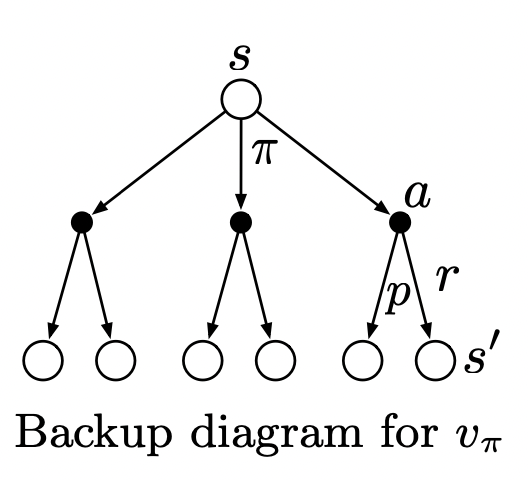
\includegraphics[scale=0.5]{images/state-backup.png}
\end{center}

The diagram expresses how the value of a state is related to the value of subsequent (possible) states. Each action can lead to one of many possible states and the value of the root state is the weighted average of these values. It is called a backup diagram because of how information flows from successor states back to the root state.

\section{Optimal Policies and Value Functions}
We need some way to compare policies; this is done through the ordering $\pi \geq \pi' \iff v_\pi(s) \geq v_{\pi'}(s) \forall s \in \mathcal{S}$. For finite MDPs there is a finite number of policies and thus some policy $\pi_*$ such that $\pi_* \geq \pi \forall \pi$. There may be multiple, but they all share the same state-value function (due to uniqueness under Bellman) called $v_*$. Similarly, there exists a unique $q_*$:

\begin{equation}
	\label{eqn:optimal-q}
	q_*(s,a) = \mathbb{E}[R_{t+1} + \gamma v_*(S_{t+1}) | S_t = s, A_t = a]
\end{equation}

Using \autoref{eqn:state-bellman}:

\begin{equation}
	\label{eqn:optimal-v-bellman}
	v_*(s) = \max_{a} \sum_{s',r} p(s',r|s,a) \left[r+\gamma v_*(s')\right]
\end{equation}


\begin{equation}
	\label{eqn:optimal-q-bellman}
	q_*(s,a) = \sum_{s',r} p(s',r|s,a) \left[r+\gamma\max_{a'}q_*(s',a')\right]
\end{equation}

Intuitively, this is because the optimal value is the expected return of taking the optimal action from $s$ plus the optimal value of the state you would end up in. This is represented in a backup diagram by drawing an arc across the edges to represent `max'.

Once we have $v_*$, the optimal policy is easy to find - any policy that assigns nonzero probabilities only to the actions that give the maximum in \autoref{eqn:state-bellman}. Similarly, if we have $q_*$ the optimal policy is that which assigns nonzero probability only to actions $a_*$ such that $a_* = \text{argmax}_{a}q(s,a)$.

Problems with directly computing $v_*$:

\begin{itemize}
	\item Dynamics $p(s',r | s,a)$ may not be known
	\item If $|\mathcal{S}|$ is large then it may be infeasible to solve all the linear equations
	\item The problem may not be Markovian
\end{itemize}


\chapter{Dynamic Programming}
Assuming we have a perfect model of the environment, we can essentially use the Bellman equation \autoref{eqn:state-bellman} as an update rule for some estimate of $v_*$ or $q_*$ respectively. This is the theoretical basis for many practical algorithms even though it is not very practical on its own.


There are three problems that need to be solved. The first \textbf{prediction} or \textbf{evaluation}: given a policy $\pi$, what is $v_\pi$? Second is \textbf{improvement} given $\pi$ and $v_\pi$ how do we derive $\pi' \ge pi$? Finally the \textbf{control} or \textbf{iteration} problem - how do we manage the process of evaluation and iteration?

\section{Evaluation (or Prediction)}
The most straightforward method is called \textbf{iterative policy evaluation}. We initialize $v_0(s)$ arbitrarily for all states except set the value of terminal states to 0 and then do:

\begin{equation}
	\label{eqn:iterative-policy-eval}
	v_{k+1}(s) = \sum_{a}\pi(a|s)\sum_{s',r}p(s',r|s,a)[r+\gamma v_k(s')]
\end{equation}

This is called a `sweep' through the state space. The update can be done with two value vectors or in-place; in-place usually converges faster. We detect convergence by computing $\delta = \max(\delta, |v_{k+1}(s) - v_k(s)|$ for each state and stopping when it goes below a threshold.


\section{Policy Improvement}
Note that this section only considers deterministic policies, but analogous results are possible for stochastic ones. If we have $\pi, v_\pi(s)$ we can apply the \textbf{policy-improvement theorem} (\autoref{eqn:policy-improvement-theorem}) to prove the following intuitive result: If it would be better to select some action $a$ in state $s$ once and thereafter follow $\pi$ than it would be to follow $\pi$ forever, then it would be better to always select $a$ in state $s$.

\begin{equation}
	\label{eqn:policy-improvement-theorem}
	q_\pi(s,\pi'(s)) \geq v_\pi(s) \ \ \forall s \in \mathcal{S} \implies \pi' \geq \pi
\end{equation}

Therefore, we can construct a new policy $\pi'$ by being \textit{greedy} with respect to $q_\pi$ and are guaranteed that this is better than the original policy.


\section{Policy Iteration (or Control)}
Combining the processes in the previous two sections allows us to converge towards an optimal policy. Simply start with any policy, evaluate it, improve it, evaluate the improved policy, and continue. We can check for policy convergence by seeing if any actions have changed (in the deterministic case) or that the KL divergence has bottomed out (in the stochastic case).

A special case of policy iteration, known as \textbf{value iteration} combines the evaluation and improvement by replacing $\pi$ in \autoref{eqn:iterative-policy-eval} with a max over the actions and performing only one state-space sweep (or, equivalently, by turning the Bellman \textit{optimality} in \autoref{eqn:optimal-v-bellman} into an update):

\begin{equation}
	\label{eqn:value-iteration}
	v_{k+1}(s) \equiv \max_{a}\sum_{s',r} p(s',r | s,a)[r+\gamma v_k(s')]
\end{equation}

\section{Asynchronous DP}
Asynchronous DP is simply DP that does not perform systematic sweeps over the state space. Instead, it updates the values of states in some arbitrary order - maintaining convergence so long as it eventually keeps updating every state. For example, asynchronous value iteration uses \autoref{eqn:value-iteration} only once in each iteration step (e.g. on a state that was actually visited by some random policy). The main benefit is that we have some more flexibility and can focus on states that are more important - and update the policy while actually experiencing the MDP.

\section{Generalized Policy Iteration}
GPI is an abstraction of the processes described above. In GPI we have two processes: one updating the value function for a policy, and the other making the policy greedy with respect to the current value function.


\chapter{Monte-Carlo Methods}\label{sec:Monte-Carlo Methods}
Monte-Carlo methods allow us to learn value functions and compute optimal policies \textit{without} the dynamics of the environment. We average returns received along trajectories and use this information to update state value functions.

\section{Prediction}
Note that the expectation of some function over random variables can be approximated by the sample mean of that function over samples of those random variables. In this case, the random variables are the sequence $R_t$ whose distribution depends on $\pi$ and the function is the (discounted) return $G_t$ in some starting state $s_0$:

\begin{equation}
	\label{eqn:mc-update}
	V_\pi(s_0) = \mathbb{E}[G_t | S_t =s_0] = \frac{1}{N} \sum_{i=1}^{N}G_i
\end{equation}

Where $G_i$ is the return we got in iteration $i$. An iteration involves running through the MDP according to $\pi$ starting at $s_0$ until we reach a terminal state.

When we perform an iteration, we may visit $s_0$ multiple times. In \textbf{first-visit} MC we get exactly 1 $G_i$ in each iteration, corresponding to the overall return of that iteration (which started in $s_0$). In \textbf{every-visit} MC we may get multiple $G_i$ in the iteration, corresponding to the returns following each visit to $s_0$ in the iteration. \textbf{Both} first and every visit MC converge to $v_\pi$ so long as we visit every state infinitely often - this is because the sample mean is an unbiased estimator of $G_t$.

The backup diagram for Monte-Carlo would be the full trajectory up to the terminal state and starting at $s_0$.

Monte-Carlo methods do not \textbf{bootstrap} because the estimate for one state does not depend on the estimate for any other state (it only uses the actual experienced rewards starting at a given state).

Advantages over DP:

\begin{itemize}
	\item Even when we know the full description of the environment, the exact probabilities $p(s',r|s,a)$ may be difficult to compute (e.g. in blackjack). Monte-Carlo does not require these
	\item Monte-Carlo can learn from actual and simulated experience
	\item The computational expense does not depend on $|\mathcal{S}|$
\end{itemize}

\subsection{Exploring Starts}
Deterministic policies may make it difficult to use MC methods to compute $q_*(s,a)$ as they cannot visit every possible action in a given state. To address this, we can specify that episodes start in a random $(s_0, a_0)$ pair to ensure that every state and action pair is visited infinitely often. This is just a trick, and the better way to do this would be to use stochastic policies.

\subsection{On-Policy Prediction}
Removing the assumption of exploring starts introduces the concepts of \textbf{off-policy} and \textbf{on-policy} methods. In \textbf{on-policy} methods, we still evaluate $v_pi$ but ensure that we still visit every action. For example, we may use 'eternally soft' $pi(a|s) > 0$ policies. We may also use $\epsilon$-soft policies (note that $A^*=\text{argmax}_{a}Q(s,a)$):

\begin{equation}
	\label{eqn:e-soft-policy}
	\pi(a|s) = \begin{cases}
 		\frac{\epsilon}{|\mathcal{A}(s)|} & a \neq A^*\\
 		1 - \epsilon + \frac{\epsilon}{|\mathcal{A}(s)|} & a = A^*
 	\end{cases}
\end{equation}

Note that using an $\epsilon$-greedy policy in this method will converge to the optimal \textit{$e$-soft} policy (\textbf{not} the overall optimum).

\subsection{Off-Policy Prediction - Importance Sampling}\label{sec:importance-sampling}
In \textbf{off-policy} control, we seek to learn the values for an optimal policy, but must behave in a non-optimal way in order to explore all actions. On-policy is a compromise - it behaves close to optimally to avoid addressing this problem.

We have \textit{two} policies: the behaviour policy $b(a|s)$ and the target policy $\pi(a|s)$. $b$ is usually some exploratory policy while $\pi$ is usually the deterministic greedy policy. Note the following

\begin{align}
	\mathbb{E}_p[f(X)] = \sum_{x \in \text{Val}(X)} p(x)f(x) = \sum_{x \in \text{Val}(X)} q(x) \frac{p(x)}{q(x)}f(x) = \mathbb{E}_q\left[\frac{p(X)}{q(X)}f(X)\right]
\end{align}

Similarly, we can compute $v_\pi(s)$ using $v_b(s)$ using:
\begin{equation}
	\label{eqn:importance-sampling-ratio}
	\rho_{t:h} \equiv \prod_{k=t}^{\min(h,T-1)}	\frac{\pi(A_k|S_k)}{b(A_k|S_k)}
\end{equation}

\begin{equation}
	\label{eqn:importance-sampling-value}
	v_\pi(s) = \mathbb{E}_b\left[\rho_{t:T-1}G_t | S_t = s\right]
\end{equation}

By behaving according to $b$ and computing the expectation in \autoref{eqn:importance-sampling-value} using sample means weighted by the product, we can converge to $v_\pi$.



\section{Improvement}
We simply make $\pi$ greedy with respect to $Q_\pi$ as before.

\section{Control}
On policy control is the same idea as GPI. Off-policy control is achieved in much the same way, but using the estimate of $V_\pi$ as discussed in \autoref{sec:importance-sampling}


\section{General Remarks}
Monte-Carlo is sort of like DFS. Information flows from root states to leaf nodes one step at a time, so the best case for updating the value of the tree is proportional to the depth of the tree.

\chapter{TD-Learning}\label{sec:TD-Learning}

Temporal-Difference (TD) learning combines concepts from DP and MC. TD updates value estimates based on other estimates - that is, it \textbf{bootstraps} like DP. TD does not require the environment dynamics and can learn from experience like MC.

\section{TD Prediction}
The simplest update, known as TD(0) or \textbf{one-step} TD:

\begin{equation}
	\label{eqn:td-0}
	V(S_t) \xleftarrow{} V(S_t) + \alpha\left[R_{t+1} + \gamma V(S_{t+1}) - V(S_t)\right]
\end{equation}

This is in contrast with \autoref{eqn:mc-update} (the target is $R_{t+1} + \gamma V(S_{t+1})$ instead of $G_t$). DP is an estimate because it uses the estimate $V(S_{t+1})$. MC is an estimate because it estimates $\mathbb{E}[G_t]$ using the sample mean. TD is an estimate for both reasons. It combines the \textbf{sampling} of MC with the \textbf{bootstrapping} of DP.

TD is guaranteed to converge to $v_\pi$ provided sufficiently small $\alpha$. TD is implemented as an \textbf{online} algorithm and thus can update values more often. It is not clear whether TD converges faster than MC in theory, but TD methods are generally preferable.

\section{On-policy TD Control: SARSA}\label{sec:SARSA}
\begin{itemize}
	\item On-policy TD: estimate $q_\pi$ for current $\pi$ while updating $\pi$
	\item Convergence: depends on how $\pi$ relates to $Q$
	\begin{itemize}
		\item $\pi$ must converge to greedy in the limit (can be acheived by slowly decreasing $\epsilon$)
	\end{itemize}
\end{itemize}

\begin{equation}
	\label{eqn:SARSA}
	Q(S_t, A_t) \xleftarrow{} Q(S_t, A_t) + \alpha \left[ R_{t+1} + \gamma Q(S_{t+1},A_{t+1}) - Q(S_t, A_t) \right]
\end{equation}

\section{Off-policy TD Control: Q-Learning}\label{par:Q-Learning}
\begin{itemize}
	\item Off-policy TD: Q-learning directly learns $q^\ast$ while behaving via $\pi$
	\item Convergence: behaviour $\pi$ eventually visits all (S,A) infinitely often
	\begin{itemize}
		\item $\epsilon$-greedy not the only possibility
	\end{itemize}
\end{itemize}


\begin{equation}
	\label{eqn:Q-Learning}
	Q(S_t, A_t) \xleftarrow{} Q(S_t, A_t) + \alpha \left[ R_{t+1} + \gamma\max_{a}Q(S_{t+1},a) - Q(S_t, A_t) \right]
\end{equation}


The idea here is that we run this algorithm for N episodes, or until we detect that $Q$ has converged. Then we have 'learned' the optimal policy $\pi_\ast$ and can begin acting according to it. This is important as this is also what DQN (see \autoref{sec:dqn}) does.

\section{Expected SARSA}\label{par:EXPSARSA}
\begin{itemize}
	\item Can be used on or off policy
	\begin{itemize}
		\item When $\pi_{\text{target}}$ is greedy and $\pi_{\text{behaviour}}$ is exploratory, it is the same as Q-Learning (as an exercise, confirm this with \autoref{eqn:EXPSARSA})
	\end{itemize}
	\item Eliminates the \textbf{variance} added by randomly selecting $A_{t+1} \sim \pi$
	\item Can set $\alpha=1$ in deterministic environments as randomness is only from the policy which is removed through taking the mean
	\item More computational complexity, but likely to outperform Q-Learning and SARSA
\end{itemize}

This algorithm subsumes Q-Learning and improves upon SARSA by removing the variance associated with the random selection of the next action. Because of this, it is likely to perform better and on a wider range of $\alpha$ while providing the same or better convergence guarantees than the other two.

\begin{equation}
	\label{eqn:EXPSARSA}
	Q(S_t, A_t) \xleftarrow{} Q(S_t, A_t) + \alpha \left[ R_{t+1} + \gamma \sum_{a \in \mathcal{A}}\pi(a|S_{t+1})Q(S_{t+1},a) - Q(S_t, A_t) \right]
\end{equation}

\section{Maximization Bias}\label{sec:double-q-learning}
Using the maximum over estimates as the estimate of the maximum (as done in Q-learning and Sarsa) can cause significant \textit{positive} bias known as maximization bias. The problem is that we are using the same samples to determine the max and compute the value. Instead, in \textbf{Double Q-Learning} we store two estimates, $Q_1(s,a)$ and $Q_2(s,a)$ and use the maximum over the values of one to update the values of the other:

\begin{equation}
	\label{eqn:double-q-learning}
	Q_x(S,A) \xleftarrow{} Q_x(S,A) + \alpha\left[R + \gamma Q_y(S, \text{argmax}_aQ_x(S, a)) - Q_x(S,A)\right]
\end{equation}

Where we randomly swap between $(x, y) = (1, 2)$ and $(2, 1)$. We can do the same thing to make double SARSA or double Expected-SARSA.


\chapter{N-step Bootstrapping}
We can view Monte Carlo methods (\autoref{sec:Monte-Carlo Methods}) and One-step TD (\autoref{sec:TD-Learning}) as being on a spectrum. MC is sort of like TD done over the whole trajectory of an episode. Since the number of steps that MC uses, it can be considered `$\infty$-step TD`.

\section{Prediction: N-Step TD}
As an intermediate between One-step TD and $\infty$-step TD (MC), in N-step TD we use the first N observed rewards plus the \textit{estimated} value of the state N steps later. To do this, it is useful to define the N-step return:


\begin{equation}
	\label{eqn:n-step-return}
	G_{t:t+n} = \gamma^nV_{t+n-1}(S_{t+n}) + \sum_{k = 0}^{n-1}\gamma^kR_{t+1+k}
\end{equation}

Note that $V_{t}$ is the estimate of $v_\pi$ at time $t$. You can think of the $V_{t+n-1}$ term as `accounting' for the missing observed rewards $R_{t+n+1}...R_{T}$ for an episode that ends at time $T$. Using this, we can write down the n-step TD update:

\begin{equation}
	\label{eqn:n-step-td}
	V_{t+n}(S_t) = V_{t+n-1}(S_t) + \alpha [ G_{t:t+n} - V_{t+n-1}(S_t)] \ \ \ 0 \le t < T
\end{equation}

N-step TD can be proved to converge for all N. As a reminder, this is just about estimating $v_\pi$ since we are considering the prediction problem. We must now look at how to perform control.

\section{Control: N-Step SARSA}
This is a generalization of SARSA (\autoref{eqn:SARSA} is `SARSA(0)'). As expected, it is \textbf{on-policy}. We use a modified definition of N-step return to use action values instead, and then use a policy that is $\epsilon$-greedy with respect to Q:

\begin{equation}
	\label{eqn:n-step-sarsa-return}
	G_{t:t+n} \equiv \gamma^n Q_{t+n-1}(S_{t+n}, A_{t+n}) + \sum_{k=0}^{n-1} \gamma^{k}R_{t+1+k}
\end{equation}

Therefore our update is

\begin{equation}
	\label{eqn:n-step-sarsa-update}
	Q_{t+n}(S_t,A_t) \equiv Q_{t+n-1}(S_t,A_t) + \alpha[G_{t:t+n} - Q_{t+n-1}(S_t,A_t)]
\end{equation}

We can also do N-step Expected SARSA by redefining $G_{t:t+n}$:

\begin{equation}
	\label{eqn:n-step-expected-sarsa-return}
	G_{t:t+n} \equiv \gamma^n \left(\sum_{a}\pi(a|S_{t+n})Q_{t+n-1}(S_{t+n},a)\right) + \sum_{k=0}^{n-1} \gamma^{k}R_{t+1+k}
\end{equation}



\section{Control: Off-Policy}
We simply use the important sampling ratio from \autoref{eqn:importance-sampling-ratio}:


\begin{equation}
	\label{eqn:n-step-off-policy-update}
	Q_{t+n}(S_t,A_t) \equiv Q_{t+n-1}(S_t,A_t) + \alpha\rho_{t+1:t+n}[G_{t:t+n} - Q_{t+n-1}(S_t,A_t)]
\end{equation}

We can then use the policy behaviour $b$ for K episodes and train the value function for the greedy policy $\pi$.

\section{Eligibility Traces}

Eligibility traces are a clever way to unify TD and MC in a computationally efficient manner. They solve the credit assignment problem by keeping a memory of visited states whose \textit{eligibility} or share in credit decrements with every step they are not revisited.

\subsection{Credit-Assignment Problem}
When we reach some state and receive a nice reward, how do we determine which pairs $(S_i, A_i)$ are most responsible for getting us here? This is the \textbf{credit assignment} problem. Monte Carlo gives \textbf{equal credit} to all the pairs that got us here. N-step TD only immediately gives credit to the pair that occurred N steps before a reward (e.g. TD(0) only credits the (s,a) that happened right before the reward).

\subsection{Lambda-Return and Lambda-TD}

What if instead of selecting a fixed N for N-step algorithms we took some sort of weighted average of them? Turns out this is good and \textbf{guaranteed} to converge so long as the weights are positive and sum to 1. TD($\lambda$) uses weights $(1-\lambda)\lambda^{n-1}$, $\lambda \in [0, 1)$ to weight each n-step return; that is, its target is the $\lambda$-return

\begin{equation}
	\label{eqn:lambda-return}
	G_t^\lambda = (1-\lambda)\sum_{n=1}^\infty \lambda^{n-1} G_{t:t+n}
\end{equation}


\subsection{Eligibility Trace Vector}
In the lectures, we use the notation that we have an array $\epsilon[s]$ that stores the 'credit' for each state. In every iteration, we set $\epsilon[s]=1$ for the current state $s$, and set $\epsilon[s'] = \lambda\epsilon[s']$ for every other state $s'$. Then, the reward to apportion to each state in $\epsilon$ is $R_t \cdot \epsilon$. When an element in the vector goes below a threshold, we delete it from the vector.

\chapter{Value Function Approximation}\label{sec:vfa}
Thus far we have assumed we can represent the values of $Q_\pi$ or $V_\pi$ for all states $s \in \mathcal{S}$. This is not feasible for enormous spaces or high-dimensional ones. Instead we use the approximations

\begin{align}
	\label{eqn:vfa-state-value}
	\hat{v}_\pi(s ; \vec{w}) &\approx v_\pi(s)\\
	\hat{q}_\pi(s, a ; \vec{w}) &\approx q_\pi(s, a)
\end{align}

Technically $\vec{w}$ doesnt really have to be a vector - it could be any information that affects the value of $\hat{v}$, but a vector is usually used since it allows us to apply calculus to minimize the error in this estimation.

The goal is to \textit{learn} the weight vector that minimizes some error between $\hat{v}_\pi(s; \vec{w})$ and $v_\pi(s)$ (the latter is the \textit{true} state value). In general, the approximated function may be any function of the weights however there are a few common cases that work well. In particular, we normally use \textbf{differentiable} functions since a typical assumption is that the value of \textit{nearby} states is related to the value of the current state. Thus when we modify a weight, it affects a \textit{range} of states in a smooth way.

We can conceive of all the algorithms hitherto considered as producing \textit{training examples} $s \xrightarrow{} u$. For example, in first-visit MC we are training on $s \xrightarrow{} G_t$ - in the tabular case we would directly move the value of the state towards $G_t$, but in VFA we smoothly adjust the weight to reduce the error on this example.

\section{Linear VFA}
We assume that the state is some vector of \textbf{features} $\vec{s}$. For example in 3-D space the features could be the $x, y$, and $z$ coordinates. $\vec{w}$ is a vector of parameters for the function. In \textbf{linear value-function approximation} we use the general form given by \autoref{eqn:linear-vfa}.

\begin{equation}
	\label{eqn:linear-vfa}
	\hat{v}_\pi(\vec{s};\vec{w}) = \vec{w}^T \vec{s} = \sum_{i=1}^{n} w_is_i
\end{equation}


\section{Prediction}

\subsection{Objective Function}\label{sec:vfa-objective-function}
The implicit goal of tabular methods was to eventually converge - reduce the error $max|V_\pi(s) - v_\pi(s)|$ to 0. Since we by definition have fewer weights than states (otherwise there would be no point in approximating), we \textbf{cannot} generally expect there to be a way to reduce this error to 0. Instead we define a new \textbf{prediction objective} to minimize:

\begin{align}
	\label{eqn:vfa-objective}
	\mathcal{J}(\vec{w}) &= \mathbb{E}_\pi\left[\bigg(v_\pi(s) - \hat{v}(s;\vec{w})\bigg)^2\right]\\
		\label{eqn:vfa-objective-density}
		&= \sum_s \mu(s) \left[\left(v_\pi(s) - \hat{v}(s;\vec{w})\right)^2\right]
\end{align}

Note that \autoref{eqn:vfa-objective-density} includes a term $\mu(s)$ which is simply the density at which the state $s$ is visited if we follow $\pi(a | s)$. It is sort of like an 'importance' measure of the value of that given state (states we visit often should have lower error).

The textbook (equation 9.1) uses the form of \autoref{eqn:vfa-objective-density} without reference to \autoref{eqn:vfa-objective}, as it assumes $\mu(s)$ can be any measure of how important state values are.

\textbf{There is no reason to believe that this is the best objective function}. This goal just seems like a good one - the real goal is to find a better policy. Regardless, it is the implicit objective of all methods considered from here.

For non-linear $\hat{v}$, the best we can usually hope for is to converge to a \textbf{local minima} of $\mathcal{J}(\vec{w})$, though ideally it would be global.

\subsection{Optimization}
Now the question is how to actually reach a local minima? Obviously this will involve some differentiation - but what datapoints should we use and when, and what should the step size be?

\subsubsection{Stochastic Gradient Descent (SGD)}
Recall that the gradient of a function $\nabla F(\vec{x})$ is a vector $\langle \frac{\partial F}{\partial x_1}, \frac{\partial F}{\partial x_2}, ..., \frac{\partial F}{\partial x_n}\rangle$. Like the ordinary derivative, this vector points in the direction that would locally \textbf{increase} the value of $\vec{x}$, so to minimize $F$ we should step in the negative gradient direction.

\autoref{eqn:sgd} shows us the update to use. Note that the $\frac{1}{2}$ factor could have just been absorbed into $\alpha$, it's just there so the result has a nice form.

\begin{align}
	\vec{w} &\xleftarrow{} \vec{w} - \frac{1}{2}\alpha \nabla_{\vec{w}} \left[ v_\pi - \hat{v}_\pi\right]^2\\
		\label{eqn:sgd}
		&= 	\vec{w} - \alpha\left[ v_\pi - \hat{v}_\pi \right] \nabla_{\vec{w}}\hat{v}_\pi
\end{align}

What makes it stochastic? This update is performed on a single $(s, v_\pi(s))$ pair. Note that we can replace $v_\pi$ with some unbiased estimate of it, called $U_t$ - with first-visit Monte Carlo this would be $U_t = G_t$.

Performing the derivative of \autoref{eqn:sgd} in the linear case gives us a simple form because we simply need to multiply the error term by the example's state vector:

\begin{equation}
	\label{eqn:linear-sgd}
	\nabla_{\vec{w}} \hat{v}_\pi(\vec{w}) = \nabla_{\vec{w}} \vec{w}^T\vec{s} = \vec{s}\ \nabla_{\vec{w}}\vec{w}^T = \vec{s}
\end{equation}

\subsection{Semi-Gradient Methods}\label{sec:semi-gradient-methods}
\textbf{Bootstrapping targets are not unbiased estimators}. We cannot achieve convergence guarantees using DP or TD($\lambda$) bootstrapping targets since their values depend on the current weight vector - making them biased. Using these estimators in \autoref{eqn:sgd} only factors in how the weight affects the error but not the value estimate - thus if we do it anyway it is called a \textbf{semi-gradient} method.



\section{VFA Coding (`Shallow' Learning)}
The feature vector $\vec{s}$ (also written $\vec{x}(S_t)$ in the textbook, as a way to decouple it from the state) is actually something we choose prior to letting the agent learn. It is a useful way for us to inject prior knowledge about a given problem, especially in the case of linear VFA. In linear VFA, we have no way to represent \textit{interactions} between state features because there are no 'cross-terms' in \autoref{eqn:linear-vfa}. Instead, we \textit{choose} the features to represent any state interactions we think are useful for the problem.

An example is the pole-balancing problem. Here, the angular velocity at which the pole is moving is good \textit{depending} on the angle. If the angle is low, a high velocity is fine (it is self-correcting). If the angle is high, a high velocity is bad since it is likely falling. So we might choose a feature $s_i = \omega \cdot \theta$ to represent the product of these two whose weight can then be adjusted.

\subsection{Coarse Coding}
One way to select features in a continuous space (e.g. 2D or 3D) is to have $n$ possibly overlapping circles. When the \textit{state} (which is technically the exact location of the point in space) is in a circle $c_i$, then $s_i = 1$ otherwise $s_i = 0$. Features like this are called \textbf{coarse coding}, though they may be as fine-grained as you like.

Remember, the goal is to make the number of features much less than $|\mathcal{S}|$. We also want to inject some prior information through the selection of features. Coarse coding provides both of these. Making the circles bigger essentially tells the agent to \textbf{generalize} over a wider region, and we can even choose irregular circles if we know a particular spot needs finer-grained discrimination

\subsection{Tile Coding}
Tile coding is a type of coarse coding, where instead of circles we use $n$ layers of grids each with a slight offset relative to the others. On a digital computer, it is much more computationally efficient to find the singular active region in each grid than to compute the value of $c_i$ in circular coding.

\subsection{Hand-Coded Tilings}
In general, we can choose whatever shapes we like to make the agent generalize in particular directions (or give the agent the \textit{option} to generalize in a given direction) or couple regions together. This should be done in some sensible way based on the problem at hand.


\section{Neural Networks}\label{sec:neural-networks}
This section is sort of optional so long as you get the basic idea of neural networks. From the perspective of this course, they are simply a biologically-inspired nonlinear value-function approximator.

\subsection{Neuron}
The basic unit is the neuron, which takes in features $\{x_1...x_d\}$, computes $net = \sum w_ix_i$ and outputs $\sigma(net)$ where $\sigma$ is the \textbf{activation function}. Usually $\sigma$ is the sigmoid function given by \autoref{eqn:sigmoid} (with the nice property given by \autoref{eqn:sigmoid-deriv})

\begin{align}
	\label{eqn:sigmoid}
	\sigma(x) &= \frac{1}{1 - e^{-x}}\\
	\label{eqn:sigmoid-deriv}
	\frac{d\sigma}{dx} &= \sigma(x)(1-\sigma(x))
\end{align}

\subsection{Net Activation}

If we compose layers of neurons where layer $j$ has weights $w_{ij}$ we can decide what values of a layer get propagated to which neurons in the next and we thus have a neural network.

\subsection{Universal Approximation Theorem}
Don't need to know the details, but essentially guarantees that a fully-connected neural network can approximate any function (under some conditions on the size).

\subsection{Gradient Descent}
Given an input-output example, we can use an optimizer to tell us how to update the weights. The updates can be batched for efficiency. Note that Stochastic Gradient-Descent isn't the only option - Adam and LBFGS are some other names.

\subsection{Problems}

\begin{itemize}
	\item Overfitting
	\item Inefficiency with time-series or image data
	\item Overfitting
	\item Overfitting
	\item Good at interpolation but not extrapolation. A few techniques can address this
	\begin{itemize}
		\item Separate data into $\sim70\%$ training data, $10\%$ validation to see how well it is doing, and use the remaining data to test at the end
		\item Dropout: randomly drop edges in the network. This creates some sets of nodes that 'specialize' and allows information to be spread. Usually done by specifying a probability $p$ that any given edge will be dropped
	\end{itemize}
	\item Catastrophic Forgetting: if we suddenly start sampling from a different distribution for example data (e.g. nonstationary problem), we will forget how to solve the original problem. How can we allow for learning new distributions? Segmented networks might be an option
\end{itemize}

\textbf{Regularization} methods aim to decrease the generalization error while not affecting the training error. That is, they punish overfitting. Dropout is one example of this, some other methods include dataset augmentation, and L1/L2 norm regularization.

\subsection{Architecture}
There are quite a few different approaches to designing the connectivity of networks, which usually depends on the \textit{type} of data we are looking at (images? time-series? spatially-structured data?). LSTM (Long Short-Term Memory) uses time as a variable to identify patterns over and is thus used in ordered data (time-series or language). CNN (Convolutional Neural Networks) perform a convolution which mixes local spatial data together, which is good for images or other spatially structured data.


\chapter{Deep Reinforcement Learning}
\section{Overview}
As discussed in \autoref{sec:neural-networks}, we can use neural networks as value-function approximators. In general, NNs minimize some \textbf{loss function}, which in our case is the difference $Target - Estimate$.

\section{Deep Q-Network (DQN)}\label{sec:dqn}

Recall the Q-Learning of \autoref{eqn:Q-Learning}. It uses the experienced reward and the \textit{maximum} of the reward estimates of adjacent states to update the current $(S, A)$ pair. Deep Q-Network uses a neural network to approximate Q. For Atari, the network is two convolutions followed by two dense layers the last of which outputs a one-hot encoding of the direction to move the joystick.

Recall also in \autoref{sec:semi-gradient-methods} that bootstrapping targets cannot be used for gradient optimization. DQN addresses this issue in two ways: replay buffers and minibatching

\subsection{Replay Buffer}
DQN accumulates a buffer D containing $(S_t, A_t, R_t, S_{t+1})$ tuples. Note that we don't need $A_{t+1}$ because Q-Learning is off-policy and uses the update of \autoref{eqn:Q-Learning}. The size of this buffer is a \textbf{hyper-parameter}. At a time $t$ this buffer is denoted $D_t = \{e_1, ... e_t\}$ where $e_k = (S_k, A_k, R_k, S_{k+1})$.

This buffer will be randomly sampled to perform the update \autoref{eqn:sgd}. Note that $\nabla_{\vec{w}}\hat{v}_\pi$ has a known form, and in practice this uses something like \texttt{autograd} to handle arbitrary architectures.

Why does this help? One problem with using bootstrapping targets in gradient descent is that successive samples are \textit{biased}. This is because the update target depends on the policy which is derived indirectly through the current estimate $Q(s, a; \vec{w})$ and the update of \autoref{eqn:sgd} doesn't factor this in. By taking \textit{uncorrelated} samples from $D$ we mitigate this bias.

\subsection{Batching or 'Mini-Batching'}
Instead of directly performing \autoref{eqn:sgd} on each timestep, we maintain two networks. One has stable parameters $\vec{w}^-$ while the other is updated every step using that equation. Every C steps, we set $\vec{w}^- = \vec{w}$. This prevents us from having a `moving target' which increases the stability of this semi-gradient method. The number of steps $C$ at which this occurs is also a hyperparameter.

\subsection{Double DQN}

We still have the issue of maximization bias for which \autoref{sec:double-q-learning} was developed. If we use DQN to approximate both $Q_1$ and $Q_2$ we get double DQN which has been shown to be effective in practice.

\subsection{Objective}

The exact objective (or \textbf{loss}) function to minimize to use is given by \autoref{eqn:dqn} (note the connection to \autoref{eqn:vfa-objective}):

\begin{equation}
	\label{eqn:dqn}
	\mathcal{J}(\vec{w}) = \mathbb{E}_{(S, A, R, S') \sim U(D)}	\left[ \left(R + \gamma \max_{a'} Q(S', a'; \vec{w}^- ) - Q(S, a; \vec{w})\right)^2 \right]
\end{equation}

Note that $x \sim U(D)$ means sampling from a discrete uniform distribution over the set $D$.

\subsection{Prioritized Experience-Replay}
Instead of sampling from $D$ uniformly, why not prioritize samples that have a high error? We can use the absolute value of the inner term of \autoref{eqn:dqn} to do this. This value is also called the \textbf{advantage} function:

\begin{equation}
	\label{eqn:dqn-advantage}
	\mathcal{A}(a, s) = |r + \gamma\max_{a'}Q(s',a';\vec{w}^-) - Q(s,a;\vec{w})|
\end{equation}



\section{Policy Gradient Methods}\label{sec:policy-gradient}

So far we have only looked at methods that compute or estimate action or state-action values based on some policy. For example, in on-policy control (\autoref{sec:SARSA}) the policy was $\epsilon$-soft with respect to the value estimate. In deep RL we use gradients (or semi-gradients) to minimize some loss function that is proportional to the error between the estimate and true state value. We then feed the (parametrized) value function to one of our control algorithms (SARSA, Q-Learning, etc.) which determines how actions are selected and policies changed.

What if instead of adjusting $\vec{w}$ to minimize this error and then feeding it to a control algorithm, our control algorithm directly manipulated the parameters of the \textit{policy}? If that is unclear, just recall that the policy is simply some probability distribution which is just a function and can thus be approximated like any other. This gives rise to \textbf{policy gradient methods}.

As a matter of notation, we use $\vec{w}$ to denote value function parameters while $\theta$ is a vector representing policy parameters. The parameterized policy function is now written $\pi(a | s, \theta)$.

Instead of minimizing a loss function as in \autoref{sec:vfa}, we maximize a performance measure (or `objective function') $J(\theta)$ and perform gradient \textit{ascent} using \autoref{eqn:policy-gradient-ascent}. Note the connection to \autoref{eqn:sgd}.

\begin{equation}
	\label{eqn:policy-gradient-ascent}
	\theta \xleftarrow{} \theta + \alpha \widehat{\nabla J(\theta)}
\end{equation}

$\widehat{x}$ means some unbiased estimate of $x$ (the exact value is also an unbiased estimate). Some methods approximate the policy and the value function. These are the \textbf{actor-critic} methods of \autoref{sec:actor-critic}.

\subsection{Policy Approximation}
Learning the policy has a few Advantages
\begin{enumerate}
	\item The policy may converge to an optimal deterministic one. This cannot be said of e.g. SARSA (\autoref{sec:SARSA})
	\item The policy may converge to an optimal stochastic one. This cannot be said of any of the other methods discussed so far (they always get the value function for a deterministic one)
	\item Policies may be simpler to approximate than value functions
	\item Can learn continuous actions
	\item Can inject prior information about the problem by selecting a parameterization
\end{enumerate}

A few good options for parametrizing a policy include soft-max'ed preferences (\autoref{eqn:policy-approx-disc} - note the connection to \autoref{eqn:gradient-bandit}) for discrete actions and normal distributions (\autoref{eqn:policy-approx-cont}) for continuous ones.

\begin{align}
	\label{eqn:policy-approx-disc}
	\pi(a | s, \theta) &= \frac{e^{h(s, a; \theta)}}{\sum_b e^{h(s, b; \theta)}}\\
	\label{eqn:policy-approx-cont}
	\pi(a | s, \theta) &\sim \mathcal{N}(a | \mu(s; \theta), \sigma(s; \theta))
\end{align}

\subsection{Policy Gradient Theorem}\label{sec:policy-gradient-theorem}
In \autoref{eqn:policy-gradient-ascent} we need to know $\widehat{\nabla J(\theta)}$. Note that $J(\theta) = v_{\pi(a|s;\theta)}(s_0)$ for the starting state $s_0$ (for simplicity, assume that there is some fixed starting state that all episodes begin with, e.g. in mazeworld we always start at some coordinate for the task).

The problem is if we try to use \autoref{eqn:state-bellman} to find the derivative we will get stuck because we do not know the dynamics function. The policy gradient theorem gives us a way to \textbf{approximate} $\widehat{\nabla{J(\theta)}}$ in this case without needing to know the dynamics function. The theorem is given by \autoref{eqn:policy-gradient-theorem}.


\begin{align}
	\label{eqn:policy-gradient-theorem}
	\nabla J(\theta) &\propto \sum_s \mu(s) \sum_a q_\pi(s, a) \nabla_{\theta} \pi (a | s, \theta)\\
		\label{eqn:policy-gradient-theorem-exp}
		&= \mathbb{E}_\pi\left[\sum_a q_\pi(S_t, a) \nabla_{\theta} \pi (a | S_t, \theta)\right]
\end{align}

The proportionality constant does not matter as it can be absorbed into the $\alpha$ of \autoref{eqn:policy-gradient-ascent}. $\mu(s)$ is the state distribution under $\pi$ as described in \autoref{sec:vfa-objective-function}

\subsection{REINFORCE Algorithm}
REINFORCE is a Monte-Carlo approach to performing policy gradient ascent. It uses the form of the policy gradient theorem given by \autoref{eqn:policy-gradient-theorem-exp}. Since this is an expectation, we can get an unbiased estimate of it by sampling the inner value and taking the average. This would involve trying all actions in each state (which would be the \textbf{all-actions} method) - REINFORCE omits this by only using $A_t$. Details of the derivation are in the textbook (section 13.3), but the result is \autoref{eqn:REINFORCE-Exp}.

\begin{equation}
	\label{eqn:REINFORCE-Exp}
	\nabla J(\theta) \propto \mathbb{E}_\pi\left[G_t \frac{\nabla_{\theta} \pi (A_t | S_t, \theta)}{\pi(A_t | S_t, \theta)}\right]
\end{equation}

So given $\pi_\theta$, and hopefully find a nice form for $\nabla_\theta \pi_\theta$, the process is as follows. We perform an episode according to $\pi_\theta$ and compute $G_t$ by averaging (with or without discounting) the received returns starting at $t$ for each $t \in [0, T)$. Then, we compute the value $\frac{\nabla_{\theta} \pi (A_t | S_t, \theta)}{\pi(A_t | S_t, \theta)}$ for each $t \in [0, T)$. We thus have $T$ samples of the thing inside the expectation of \autoref{eqn:REINFORCE-Exp} which we can use to update $\theta$ using \autoref{eqn:policy-gradient-ascent}.


Since REINFORCE is a Monte-Carlo method, it may have high variance (unbiased does not mean zero variance!). It also may converge slowly. This can be improved using \textbf{baselines}, discussed in the next section.

\subsubsection{Baselines}\label{sec:reinforce-baseline}
As long as we subtract some function that only depends on the \textbf{state}, we add no bias to the estimate and can improve the variance and thus get faster convergence. A good choice for this is some approximation of the state value function. Given such a baselines $b(S_t)$ we use the update of \autoref{eqn:REINFORCE}. Note that since $b(S_t)$ could be 0 this is the most general form of REINFORCE.


\begin{equation}
	\label{eqn:REINFORCE}
	\nabla J(\theta) \propto \mathbb{E}_\pi\left[\left(G_t - b(S_t)\right)\nabla_\theta \ln(\pi(A_t | S_t, \theta))\right]
\end{equation}

Note: $\nabla \ln(x) = \frac{\nabla(x)}{x}$ is just a trick so we can work with log-probabilities that have better numerical properties. If we use the parameterized state value function \autoref{eqn:vfa-state-value} we can also learn \textit{its} value by using its gradient every step using $v_\pi \approx G_t$ in \autoref{eqn:sgd} ($\delta$ is the TD error):

\begin{align}
	\delta &\xleftarrow{} G_t - \hat{v}_\pi(S_t; \vec{w_t})\\
	\label{eqn:reinforce-baseline-w}
	\vec{w}_{t+1} &\xleftarrow{} \vec{w}_t + \alpha_{w} \delta \nabla_{\vec{w}} \hat{v}_\pi(S_t; \vec{w_t})\\
	\label{eqn:reinforce-baseline-theta}
	\theta_{t+1} &\xleftarrow{} \theta_{t} + \alpha_\theta \delta \nabla_\theta \ln(\pi(A_t | S_t, \theta))
\end{align}

\subsubsection{Parameter Update}

To get the full update we combine \autoref{eqn:REINFORCE} with \autoref{eqn:policy-gradient-ascent}:

\begin{equation}
	\theta_{t+1} \xleftarrow{} \theta_t + \alpha\left(G_t - b(S_t)\right)\nabla_\theta\ln(\pi(A_t | S_t, \theta))
\end{equation}

\section{Actor-Critic Methods}\label{sec:actor-critic}
Instead of simply using a learned state-value as a baseline (as in REINFORCE with baselines - \autoref{sec:reinforce-baseline}), we can use it to point the policy parameter update of \autoref{eqn:policy-gradient-ascent} in a direction that will tend to increase the value of $S_{t+1}$. We can also think of this as using the estimated state value to assess which actions are better to take from a given state.

Notice how in REINFORCE with baselines, \autoref{eqn:reinforce-baseline-theta} only uses the estimate of the value of $S_t$. In actor-critic methods, it will use the estimate of $S_{t+1}$ as well. Simply put, we can redefine the TD error to use the value estimate of the next state:

\begin{equation}
	\label{eqn:actor-critic-error}
	\delta = \delta_t = R_{t} + \gamma \hat{v}_\pi(S_{t+1}; \vec{w}) - \hat{v}_\pi(S_t; \vec{w})
\end{equation}

More generally, we can use any function for $\delta_t$ that tells us the advantage of $a$ in $s$. For example, $A_\pi(s, a) = Q_\pi(s, a) - V_\pi(s)$ tells us how action $a$ compares to the average value of actions in the given state.

\subsection{A3C and A2C}
Asynchronous Advantage Actor-Critic (A3C) was the first one to be developed \footnote[1]{Original paper available at \href{https://arxiv.org/pdf/1602.01783.pdf}{https://arxiv.org/pdf/1602.01783.pdf}}, and later it was found that the asynchronous part wasnt needed which lead to Advantage Actor-Critic (A2C).

Both algorithms use some sort of neural network to parameterize the value function and policy.

\subsubsection{A3C}
In A3C, we have a bunch of actors running in parallel. Each gets an initial copy of $\theta$ and $\vec{w}$ to work with. They perform the usual algorithm (combining \autoref{eqn:actor-critic-error} with \autoref{eqn:reinforce-baseline-w} and \autoref{eqn:reinforce-baseline-theta}) but instead of actually updating $\theta$ and $\vec{w}$, they accumulate the value on the right hand side of the latter equations. Every once in a while the actor sends these values to the root 'controller' which adds them to the global parameters. It then synchronizes its own parameters with the global ones and repeats this process.

\subsubsection{A2C}
Instead of allowing updates to occur asynchronously, the controller just waits for all agents to finish the current iteration, updates the global parameters, then runs the agent again with the new parameters. This 'batched' training works better with hardware accelerators (e.g. GPUs) where IO is the bottleneck - updates can be accumulated and then sent at once to the controller.

\section{TRPO and PPO}
\textbf{Trust-Region Policy Optimization} (TRPO) relies on the idea that taking too large of a step in policy space may result in a bad policy that prevents convergence - instead we take 'small' steps. The question is how to quantify 'small steps' and the answer is through KL divergence. Consider two policies $\pi_\theta(a | s)$ and $\pi_{\theta'}(a | s)$. They are just probability distributions, and KL divergence is a way to measure how different one probability distribution is from another (it is technically not a distance as it is not symmetric). The KL divergence is given by \autoref{eqn:KL-Divergence}.

\begin{equation}
	\label{eqn:KL-Divergence}
	\text{D}_{\text{KL}}(P|| Q) = \sum_{x} P(x) \log\frac{P(x)}{Q(x)}
\end{equation}

The objective in TRPO is to find $\text{argmax}_{\theta}J(\theta)$ subject to the constraint \autoref{eqn:trpo-constraint}
\begin{equation}
	\label{eqn:trpo-constraint}
	\mathbb{E}\left[ \text{D}_{\text{KL}}(\pi_{\theta_{\text{old}}} || \pi_{\theta}) \right] \le \delta
\end{equation}

What is $J(\theta)$ in this case? It is essentially the importance sampling ratio of using parameters $\theta$ for the policy instead of $\theta_{\text{old}}$:

\begin{equation}
	\label{eqn:trpo-objective}
	J(\theta) = \mathbb{E}_{\pi_{\theta_\text{old}}}\left[  \frac{\pi_{\theta}(a|s)}{\pi_{\theta_\text{old}}(a|s)} A_{\theta_{\text{old}}}(s, a) \right]
\end{equation}


\subsection{PPO}
TRPO uses a slightly complex $J(\theta)$ - \textbf{Proximal Policy Optimization} (PPO) simplifies this in a way that makes the constraint easier to solve. It does so by clipping the value inside the expectation of \autoref{eqn:trpo-objective}.


\section{Deterministic Policy Gradients}
In this approach, we work with a deterministic policy $\mu_theta$. The idea is that this reduces the dimensionality of the space the gradient is integrated over (no longer state and action, just state) which gives us a computational advantage over stochastic policy gradients. We must work with off-policy methods here to get exploration though.


\subsection{Deterministic Policy Gradient Theorem}
This is a deterministic analog to \autoref{eqn:policy-gradient-theorem}:

\begin{equation}
	\label{eqn:deterministic-pgt}
	\nabla_\theta J(\mu_\theta) = \mathbb{E}_{\mu_\theta} \left[ \nabla_\theta \mu_\theta(s) \left(\nabla_a Q_{\mu_\theta}(s, a)\right)\rvert_{a = \mu_\theta(s)}\right]
\end{equation}

\subsection{Deterministic Policy Gradient (DPG)}
Using \autoref{eqn:deterministic-pgt} the update we use, analogous to \autoref{eqn:policy-gradient-ascent} is

\begin{equation}
	\label{eqn:dpg-update}
	\theta_{t+1} \xleftarrow{} \theta_{t} + \alpha \nabla_\theta \mu_\theta(s) \left(\nabla_a Q_{\mu_\theta}(s, a; \vec{w})\right)\rvert_{a = \mu_\theta(s)}
\end{equation}

Note that since the gradient is taken with respect to the actions, this only works for continuous action spaces. This is fine because it is large action spaces for which this method is useful in the first place.

\subsubsection{Deep Deterministic Policy Gradient (DDPG)}
In DDPG we add some noise to the stochastic behaviour policy and use neural networks for estimation.

\subsubsection{Soft Actor-Critic (SAC)}
In this method, we include the policy entropy in $J(\theta)$ which helps with convergence and exploration. The main idea is to parameterize $\pi$ with respect to $Q$ using a softmax distribution.

\begin{enumerate}
	\item Update Q using a gradient step
	\item Take a gradient step in $\theta'$ space to minimize \autoref{eqn:sac-min}
	\item Repeat until convergence
\end{enumerate}

\begin{equation}
	\label{eqn:sac-min}
	\text{D}_{\text{KL}}\left(\pi_{\theta'} || \frac{1}{Z}e^{Q_{\pi_\theta}(s, a)}\right)
\end{equation}

Where Z is the normalizing constant for softmax.


\section{Monte Carlo Tree Search (MCTS)}
In this method, we maintain a tree of states and their values and update it for a fixed number of steps before taking an action. There are 4 steps that are repeated N times:

\begin{enumerate}
	\item Selection: starting at the root node R, recursively traverse selecting the child with highest value at each step until a leaf L is reached
	\item Expansion: given a (non-terminal) leaf, add $|\mathcal{A}|$ children corresponding to the avilable actions at this leaf, and select the first one (M)
	\item Simulation: simulate the environment from M until a terminal state is reached, which gives us a value (e.g. 1 for a win state or 0 otherwise)
	\item Backpropagation: update the values of the nodes M through R
\end{enumerate}

\subsection{Alpha-Beta Search}
At each step during simulation, alternatingly choose the best action for yourself and the best action your opponent can take (i.e. the worst action for you). This must be based on some heuristic function - the accuracy is not that important, just a way of hinting which states may be better for a given agent.

This method is difficult for games like Go where no good heuristic can be determined.

\subsection{Game Tree}
We can use something like UCB (\autoref{sec:UCB}) or a value neural network to store probabilities of actions by training on human or other AI players. We can use this to guide the growth of the 'game tree' and backpropagate the right values.

\end{document}
